\part{Mecánica Clásica}
\section{Clase 1}
\subsection{Mecánica de Newton}
Posición, velocidad, aceleración, fuerza.

Si consideramos un sistema de partículas de masa $m$
\begin{equation}
  \vec{p}_\alpha =m_\alpha \vec{\dot{x}}_\alpha,\qquad \vec{p}=\sum_\alpha \vec{p}_\alpha,\qquad \alpha=1,...,k
\end{equation}
\begin{equation}
  T=\frac{1}{2}\sum_\alpha m_\alpha \vec{\dot{x}}^2,\qquad \vec{L}=\sum_\alpha \vec{x}_\alpha\times \vec{p}_\alpha
\end{equation}
Newton estableció que a dinámica de un sistema mecánico queda	determinada por tres leyes fundamentales:
\begin{itemize}
	\item \textbf{Primera ley del movimiento:} Todo cuerpo en reposo permanecerá en reposo o en movimiento rectilíneo uniforme (MRU), a menos que una fuerza externa actúe sobre él.
	\item \textbf{Primera ley del movimiento:} Un cuerpo cambia su estado de movimiento si una fuerza actúa sobre él
	\begin{equation}
  \vec{F}=m\vec{a}
\end{equation}

\item \textbf{Tercera ley del movimiento:} A cada acción le corresponde una reacción paralela y opuesta.
\end{itemize}

Estas lees sólo son válidas en un sistema de referencia inercial (SRI). Dos SRI están relacionados por medio de una transformación de Galileo.

\begin{figure}[h!]
	\centering
	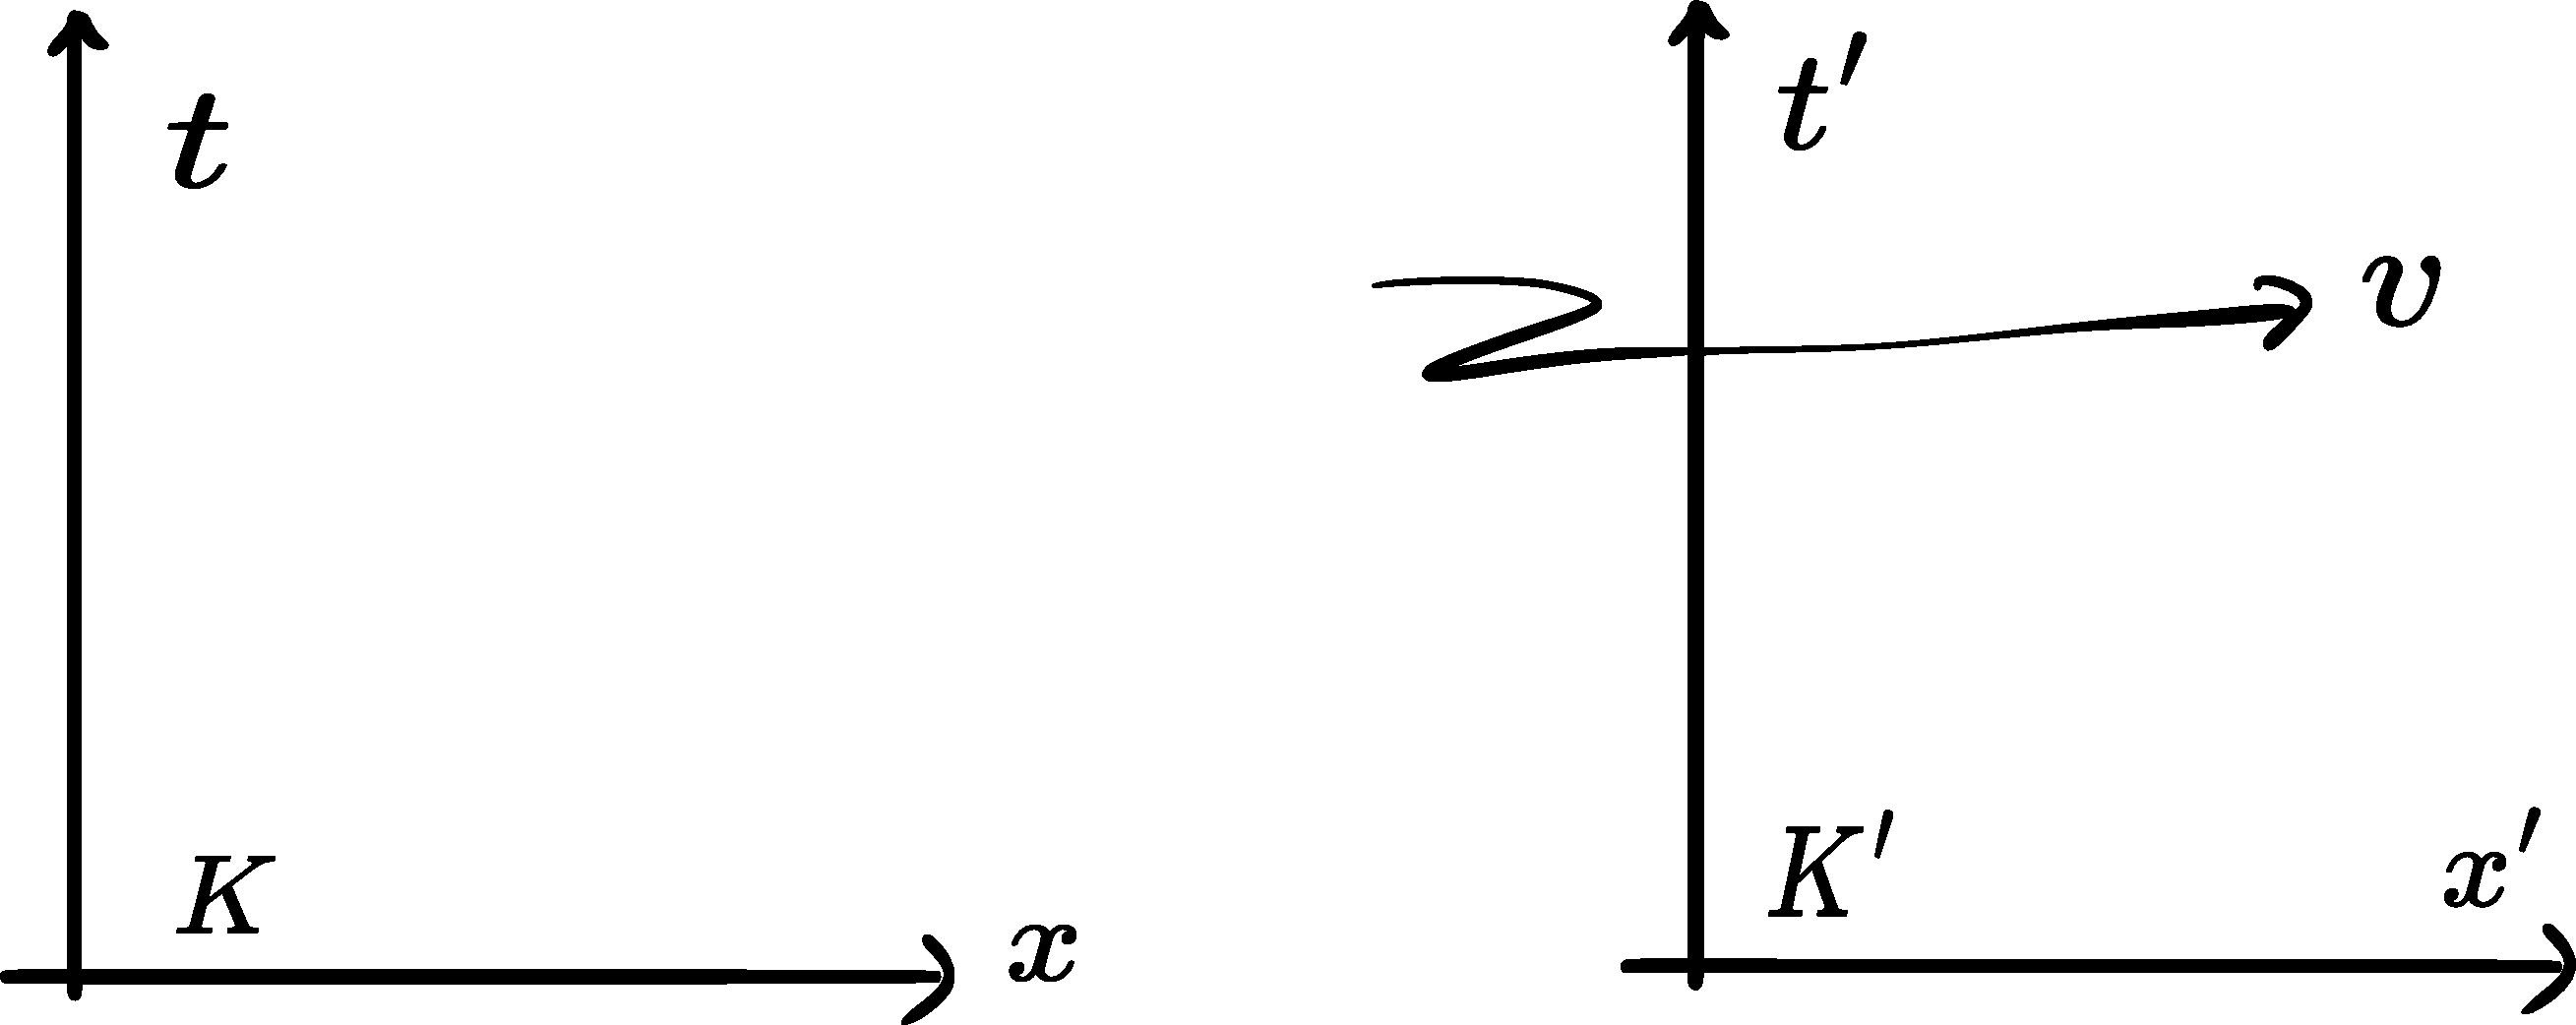
\includegraphics[scale=0.2]{fig/Galileo.pdf}
\end{figure}

\begin{align}
  x'&=x-vt\\
  t'&=t
\end{align}

Además
\begin{align}
  \vec{F}_\a &=m\ddot{\vec{x}}
\end{align}
\begin{equation}
	\implies m\ddot{\vec{x}}_\a =\dv{t}(m\dot{\vec{x}}_\a )=\dv{t}\vec{p}_\a =\dot{\vec{p}}_\a 
\end{equation}
Si las fuerzas son conservativas, se tiene
\begin{equation}
  \vec{F}_\a =-\vec{\nabla} V_\a 
\end{equation}
\begin{equation}
  \implies \boxed{\vec{\dot{p}}_\a +\vec{\nabla}V_\a =0}
\end{equation}

\subsection{Mecánica de Lagrange}
Es basada en la llamada función de Lagrange, definida como
\begin{equation}
  L(\vec{x}_\a ,\dot{\vec{x}}_\a ,t)=T(\dot{\vec{x}}_\a ,t)-V(\vec{x}_\a ,t)
\end{equation}
Lagrange introdujo el concepto de coordenada generalizada
\begin{equation}
  q_i,\quad i=1,2,...,f
\end{equation}
donde $f$ son los grados de libertad del sistema. De esta manera, se define la derivada de Euler-Lagrange como
\begin{equation}
  [L]_i=\EL=0
\end{equation}
Así, las soluciones a estas ecuaciones describen la dinámica del sistema en un espacio $f$-dimensional de coordenadas $q_i,q_2,...,q_f$.

\underline{\textbf{Nota}}: La energía cinética debe ser una función homogénea de grados dos
\begin{equation}
  T=\sum_{i,k} a_{ik}\qd_i\qd_k
\end{equation}

Notemos que una función de Lagrange dada por
\begin{equation}
  L'=L+\dv{t}B(q,t)
\end{equation}
conduce a las mismas ecuaciones del movimiento.

La libertad en la elección de coordenadas generalizadas implica que las ecuaciones de movimiento de Euler-Lagrange son \textit{estructuralmente invariantes} bajo una transofrmación de coordenadas generalizadas, es decir, bajo
\begin{equation}
  q_i\to q'_i=q'_i(q_l)\implies \qd '_i=\pdv{q'_i}{q_l}\qd_l
\end{equation}
\begin{equation}
  \pdv{\qd'_i}{\qd _l}=\pdv{q'_i}{q_l}
\end{equation}
Definiendo 
\begin{equation}
  \varphi(q_l)=\pdv{q'_i}{q_l}
\end{equation}
se tiene
\begin{equation}
  \dv{t}\varphi(q_l)=\pdv{\varphi}{q_l}\dot{q}_l
\end{equation}
luego
\begin{equation}
  \dv{t}\pdv{q'_i}{q_l}=\pdv{q_k}\left(\pdv{q'_i}{q_l}\right)\qd_k
\end{equation}
\begin{equation}\label{1.1}
  \implies \boxed{\dv{t}\pdv{q'_i}{q_l}=\pdv{q'_i}{q_k}{q_l}\qd_k}
\end{equation}
Dado que
\begin{equation}
  \qd'_i=\pdv{q'_i}{q_l}\qd_i
\end{equation}
\begin{equation}\label{1.2}
  \pdv{\qd_i}{q_l}=\pdv{q_l}\left(\pdv{\qd_i}{q_k}\qd_k\right)=\pdv{\qd_i}{q_l}{q_k}\qd_k+\cancelto{0}{\pdv{\qd_i}{q_k}\pdv{\qd_k}{q_l}}
\end{equation}
\begin{equation}
  \implies \boxed{\dv{t}\pdv{q'_i}{q_l}=\pdv{\qd_i}{q_l}}
\end{equation}
Dado que $L'(q',\qd',t)=L(q,\qd,t)$, calculemos
\begin{equation}
  \dv{t}\pdv{L'}{\qd'_k}
\end{equation}























\subsection{Acerca de la matriz Hessiana de las ecuaciones de Euler-Lagrange}
\begin{equation}
  \dv{t}\pdv{L'}{\dot{q}'_k}=\pdv{L'}{q'_k}-[L]_k\pdv{q_l}{\dot{q}_k}
\end{equation}
\begin{equation}
  \Rightarrow \pdv{L'}{q'_k}=\dv{t}\pdv{L'}{\dot{q}_k}=[L]_l\pdv	{q_l}{q'_k}
\end{equation}
\begin{equation}
\boxed{[L']_k=[L]_l\pdv{q_l}{q'_k}}
\end{equation}
La derivada de Euler-Lagrange transforma como un vector covariante bajo una transformación de coordenadas
\begin{equation}
  \mbox{Si }[L]_l=0 \Rightarrow [L']_k=0
\end{equation}


